
\chapter{Evolution Strategies}\label{ch:es}

\section{Introduction}

\bfit{Evolution Strategies (ES)} are a family of optimization algorithms developed in Germany during the 1960s, primarily by Ingo Rechenberg, Hans-Paul Schwefel, and Peter Bienert. Initially conceived for experimental optimization of hydrodynamic shapes, ES has since evolved into a robust methodology for numerical optimization, particularly in continuous domains.

While sharing common roots with Genetic Algorithms (GAs) in the broader field of evolutionary computation, ES possesses distinct characteristics.

\begin{observationblock}[ES and GAs: Similarities and Key Differences]
    \textbf{Similarities:}
    \begin{itemize}
        \item They maintain a \bfit{population} of candidate solutions.
        \item Offspring are generated primarily through \bfit{mutation}, which introduces variation.
        \item A \bfit{selection process} determines which individuals survive and/or reproduce, driving the population towards better solutions.
    \end{itemize}

    \textbf{Key Differences:}
    \begin{itemize}
        \item \bfit{Crossover (Recombination)}: While modern ES can incorporate recombination, it was not a primary operator in early ES and is often considered secondary to mutation. GAs, conversely, typically emphasize crossover.
        \item \bfit{Selection Mechanism}: ES commonly employs deterministic \bfit{truncation selection}, where only the top-ranked individuals survive or become parents. GAs often use probabilistic selection methods like roulette wheel or tournament selection.
        \item \bfit{Representation}: ES is predominantly designed for and applied to problems with \bfit{real-valued (floating-point) individuals}, whereas GAs were initially developed with binary strings and have been adapted for other representations.
        \item \bfit{Self-Adaptation}: A hallmark of advanced ES is the self-adaptation of strategy parameters (e.g., mutation strengths and directions), which are encoded within the individuals and evolve alongside the solutions themselves.
    \end{itemize}
\end{observationblock}

\section{Core Concepts and Notation}

Two key parameters define the size of the parent and offspring populations in ES:
\begin{itemize}
    \item $\bfit{\mu}$ (mu): The number of \bfit{parent individuals} selected in each generation to create offspring.
    \item $\bfit{\lambda}$ (lambda): The number of \bfit{offspring individuals} generated in each generation.
\end{itemize}

It is generally required that $\lambda \ge \mu$.

Based on how parents and offspring are managed and selected, two main ES schemes are distinguished: the $(\mu, \lambda)$-ES and the $(\mu + \lambda)$-ES.

\subsubsection{The $(\mu, \lambda)$-ES Scheme}
In the $(\mu, \lambda)-ES$ (read as "mu comma lambda ES"), the process is as follows:
\begin{enumerate}
    \item From a population of $\mu$ parent individuals, $\lambda$ offspring are generated (typically, each parent produces $\lambda/\mu$ offspring if mutation is the sole operator, or parents are selected to participate in recombination and mutation).
    \item The fitness of these $\lambda$ offspring is evaluated.
    \item The best $\mu$ individuals are selected from the $\lambda$ \textit{offspring only} to become the parents for the next generation.
    \item The $\mu$ parents from the current generation are discarded, regardless of their fitness compared to the offspring.
\end{enumerate}
This scheme is inherently non-elitist. It can allow the strategy to escape local optima more easily as fitness can temporarily decrease. However, it also risks losing the best-so-far solution if it's not re-discovered by an offspring.

\begin{figure}[H]
    \centering
    \includegraphics[width=0.6\textwidth]{assets/es-cycle-1.png}
    \caption{The lifecycle of a $(\mu, \lambda)-ES$. Selection is performed only among the offspring.}
    \label{fig:mu_lambda_es_cycle}
\end{figure}

\subsubsection{The $(\mu + \lambda)$-ES Scheme}
In the \bfit{$(\mu + \lambda)$-ES} (read as "mu plus lambda ES"), the process is as follows:
\begin{enumerate}
    \item From a population of $\mu$ parent individuals, $\lambda$ offspring are generated.
    \item The fitness of these $\lambda$ offspring is evaluated.
    \item The best $\mu$ individuals are selected from the \textit{combined pool} of the $\mu$ current parents and the $\lambda$ newly generated offspring (total $\mu + \lambda$ individuals). These $\mu$ selected individuals form the parent population for the next generation.
\end{enumerate}
This scheme is \bfit{elitist} because the best solutions found so far (parents or offspring) are guaranteed to be preserved in the next generation if they remain among the top $\mu$ individuals. This often leads to faster convergence towards local optima but can sometimes result in premature convergence if diversity is lost too quickly.

\begin{figure}[H]
    \centering
    \includegraphics[width=0.6\textwidth]{assets/es-cycle-2.png}
    \caption{The lifecycle of a $(\mu + \lambda)-ES$. Selection occurs from the combined set of parents and offspring.}
    \label{fig:mu_plus_lambda_es_cycle}
\end{figure}

\vspace{-1em}

\begin{exampleblock}[Illustrative (1,3)-ES]
    Consider a simple $(1,3)$-ES, a specific type of $(\mu, \lambda)$-ES where $\mu=1$ and $\lambda=3$.
    \begin{enumerate}
        \item Start with one parent individual.
        \item This single parent generates three offspring (e.g., by applying mutation three independent times).
        \item The fitness of these three offspring is evaluated.
        \item The single best offspring out of the three becomes the sole parent for the next generation. The original parent and the other two offspring are discarded.
    \end{enumerate}
    This process continues over several generations, with each generation showing a parent producing multiple offspring, some being discarded, and one being selected to continue. Generally, this leads to an increase in fitness over time as the population evolves toward better solutions.
\end{exampleblock}

\section{Mutation in Evolution Strategies}
Mutation is the primary engine of variation and exploration in ES, especially in simpler forms that do not use recombination.

\subsection{Properties of a Good Mutation Operator}
A well-designed mutation operator should ideally exhibit the following properties:
\begin{itemize}
    \item \bfit{Reachability:} Any point in the search space should be reachable from any other point in a finite number of mutation steps. This ensures the algorithm is not, in principle, confined to a subspace.
    \item \bfit{Unbiasedness:} The mutation operator itself should not introduce any bias towards particular regions of the search space based on fitness values. The guidance towards promising regions is the role of selection.
    \item \bfit{Scalability (Adaptability):} The "strength" or step size of the mutation should be adaptable to the characteristics of the fitness landscape. For instance, larger steps might be beneficial early in the search (exploration), while smaller steps are preferred later for fine-tuning (exploitation).
\end{itemize}

\subsection{Mutation for Different Representations}
\begin{itemize}
    \item \bfit{Binary Values:} For individuals represented as binary strings, mutation typically involves \bfit{bit-flips}, similar to GAs, where each bit has a probability of being inverted.
    \item \bfit{Real Values:} For individuals represented as vectors of real numbers $\mathbf{x} = (x_1, \ldots, x_n)$, mutation is commonly performed by adding random noise, often from a Gaussian distribution:
    $$
      x_i' = x_i + N(0, \sigma_i^2)
    $$
    Here, $x_i$ is the $i$-th component of the individual, $N(0, \sigma_i^2)$ is a random number drawn from a Gaussian (normal) distribution with mean 0 and standard deviation $\sigma_i$ (or variance $\sigma_i^2$). The $\sigma_i$ values are called \bfit{mutation strengths} or \bfit{step sizes} and are critical parameters. A key question is how to determine appropriate values for these $\sigma_i$'s.
\end{itemize}

\begin{figure}[H]
    \centering
    % Basic representation of Gaussian mutation
    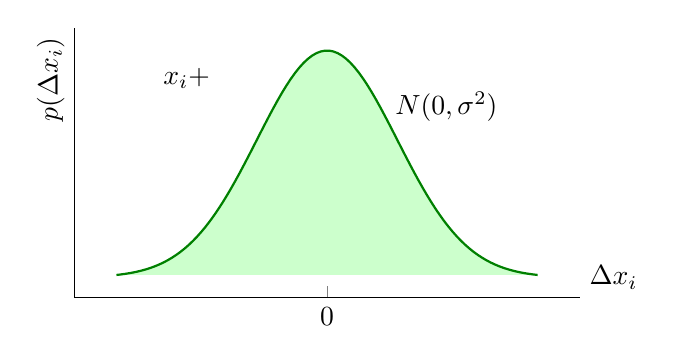
\begin{tikzpicture}
        \begin{axis}[
            no markers, domain=-3:3, samples=100,
            axis lines*=left, xlabel=$\Delta x_i$, ylabel=$p(\Delta x_i)$,
            height=5cm, width=8cm,
            ytick=\empty, xtick={0}, xticklabels={$0$},
            every axis x label/.style={at=(current axis.right of origin),anchor=west},
            every axis y label/.style={at=(current axis.north west),anchor=south east,rotate=90},
            legend pos=outer north east]
        \addplot [draw=green!50!black, fill=green!20, thick] {exp(-x^2/2)/sqrt(2*pi)};
        \node at (axis cs: 1.7, 0.3) {$N(0, \sigma^2)$};
        \node at (axis cs: -2, 0.35) {$x_i + $};
        \end{axis}
    \end{tikzpicture}
    \caption{Gaussian mutation adds a random value drawn from a normal distribution (centered at 0) to a coordinate $x_i$. The variance $\sigma^2$ controls the average step size.}
    \label{fig:gaussian_mutation}
\end{figure}

\vspace{-1em}

Setting $\mu=0$ for the Gaussian noise (i.e., $N(0, \sigma^2)$) seems natural as it ensures mutation is unbiased in direction. However, selecting the variance (or standard deviation $\sigma$) is crucial and often addressed through self-adaptation.

\subsection{Self-Adaptation of Mutation Parameters}
A powerful feature of many ES variants is \bfit{self-adaptation}, where the strategy parameters (like mutation step sizes $\sigma_i$) are not fixed but are themselves part of the individual's genotype and evolve alongside the solution variables.
\begin{itemize}
    \item An individual can be represented as a pair $\langle \mathbf{x}, \mathbf{s} \rangle$, where $\mathbf{x}$ is the vector of solution variables and $\mathbf{s}$ is a vector of strategy parameters (e.g., $\sigma_i$ values for each $x_i$, or parameters for a covariance matrix in more advanced ES).
    \item When an individual is mutated to create an offspring, its strategy parameters $\mathbf{s}$ are typically mutated first.
    \item Then, these mutated strategy parameters $\mathbf{s}'$ are used to mutate the solution variables $\mathbf{x}$ to get $\mathbf{x}'$.
    \item Selection then acts on the fitness of $\mathbf{x}'$, indirectly selecting for effective strategy parameters as well.
\end{itemize}
This allows the ES to automatically adjust its mutation behavior to suit the local topology of the fitness landscape.

\subsubsection{The One-Fifth (1/5) Success Rule}
The \bfit{1/5 success rule}, introduced by Ingo Rechenberg in the 1970s, is an early and influential heuristic for adapting a single, global mutation step size $\sigma$ in a (1+1)-ES or similar simple ES.
The rule aims to maintain a certain rate of successful mutations (those that lead to fitter offspring).
\begin{itemize}
    \item Let $p_s$ be the proportion of successful mutations (i.e., mutations that result in an offspring at least as fit as its parent) measured over a certain number of generations or mutations.
    \item The rule states:
        \begin{itemize}
            \item If $p_s > 1/5$: The success rate is too high, suggesting the step size $\sigma$ might be too small (too cautious). Increase $\sigma$.
            \item If $p_s < 1/5$: The success rate is too low, suggesting $\sigma$ might be too large (too exploratory, often overshooting optima). Decrease $\sigma$.
            \item If $p_s = 1/5$: The step size is considered optimal; leave $\sigma$ unchanged.
        \end{itemize}
    \item Operationally, this is often implemented by checking every $k$ generations (or after $k$ mutations):
    Define a constant $c \in (0,1)$, typically $0.817 < c < 1$ (e.g., $c \approx 0.85$).
        \begin{itemize}
            \item If $p_s > 1/5$, then set $\sigma \leftarrow \sigma / c$. (Since $c<1$, $1/c > 1$, so $\sigma$ increases).
            \item If $p_s < 1/5$, then set $\sigma \leftarrow \sigma \cdot c$. ($\sigma$ decreases).
            \item Otherwise (if $p_s \approx 1/5$), $\sigma$ remains unchanged.
        \end{itemize}
\end{itemize}

\begin{tipsblock}[Rationale of the 1/5 Success Rule]
    The 1/5 success rule provides a simple mechanism for controlling the balance between exploration and exploitation. A high success rate ($>1/5$) implies that the algorithm is making progress easily, possibly with steps that are too small; increasing the step size encourages broader exploration. A low success rate ($<1/5$) suggests that many mutations are detrimental, possibly because the step size is too large; decreasing it allows for finer exploitation of the current region. The value 1/5 was derived empirically and theoretically for specific model problems (e.g., the sphere model and corridor model).
\end{tipsblock}

\section{Evolution Strategies with Recombination}
While mutation is the primary search operator in ES, \bfit{recombination} (crossover) can also be incorporated, often to good effect, especially in more complex ES variants. Recombination in ES typically involves $\rho$ (rho) parent individuals to produce one or more offspring.

The notation for ES schemes is extended to include $\rho$:
\begin{itemize}
    \item \bfit{$(\mu/\rho, \lambda)$-ES}: $\mu$ parents are selected, from which groups of $\rho$ individuals are chosen to act as parents for recombination, generating $\lambda$ offspring. Selection for the next generation is from the $\lambda$ offspring.
    \item \bfit{$(\mu/\rho + \lambda)$-ES}: Similar parent selection and recombination, but selection for the next generation is from the combined pool of $\mu$ current parents and $\lambda$ offspring.
\end{itemize}

For real-valued representations, common recombination types include:

\subsection{Discrete Recombination}
Also known as \bfit{dominant recombination}. For each component (gene) $j$ of the offspring's solution vector $\mathbf{x}'$, the value is taken from one of the $\rho$ selected parent individuals, chosen randomly for that component.
$$
  x_j' = x_{p_j, j}
$$
where $p_j \in \{1, \ldots, \rho\}$ is a randomly chosen index of one of the $\rho$ parents contributing to this offspring, for each component $j$. The strategy parameters $\mathbf{s}$ can also be recombined this way.

\subsection{Intermediate Recombination}
For each component $j$ of the offspring's solution vector $\mathbf{x}'$, the value is the arithmetic average of the corresponding components from the $\rho$ selected parent individuals:
$$
  x_j' = \frac{1}{\rho} \sum_{i=1}^{\rho} x_{i,j}
$$
This tends to create offspring that lie "in between" their parents. It can be applied to both solution variables $\mathbf{x}$ and strategy parameters $\mathbf{s}$.
A common choice is $\rho=2$, where the offspring is the midpoint of its two parents, or $\rho=\mu$, where all parents in the current selection pool contribute.

\begin{exampleblock}[Recombination in Practice]
    Suppose we use $\rho=2$ parents for recombination.
    \begin{itemize}
        \item \bfit{Discrete Recombination:} For an offspring $\mathbf{x}' = (x'_1, \ldots, x'_n)$ from parents $\mathbf{p}_1$ and $\mathbf{p}_2$:
        For each $j \in \{1, \ldots, n\}$, $x'_j$ is randomly chosen to be either $p_{1,j}$ or $p_{2,j}$.
        \item \bfit{Intermediate Recombination:} For an offspring $\mathbf{x}'$ from parents $\mathbf{p}_1$ and $\mathbf{p}_2$:
        For each $j \in \{1, \ldots, n\}$, $x'_j = (p_{1,j} + p_{2,j}) / 2$.
    \end{itemize}
    Recombination can be either \bfit{global} (using one set of $\rho$ parents for all components of an offspring) or \bfit{local/component-wise} (using different parent sets for each component), with global recombination being more common in practice.
\end{exampleblock}